\begin{frame}{Summary and Contributions}
  \begin{itemize}
  \item Increasing volume of data.
  \item Network adaptation.
  \item Compute adaptation.
  \item Systematic and quantitative approach.
  \end{itemize}
\end{frame}

\begin{frame}{Current (other) and Future Work}
  \vspace{1em}
  \metroset{block=fill}
  \begin{block}{TerraSwarm Vision}
    TerraSwarm applications are characterized by their ability to
    \textit{dynamically recruit} resources such as sensors and data from the
    cloud, aggregate and use that information to make or aid decisions.
  \end{block}

  \pause
  
  \begin{figure}
    \begin{subfigure}{0.49\textwidth}
      \centering
      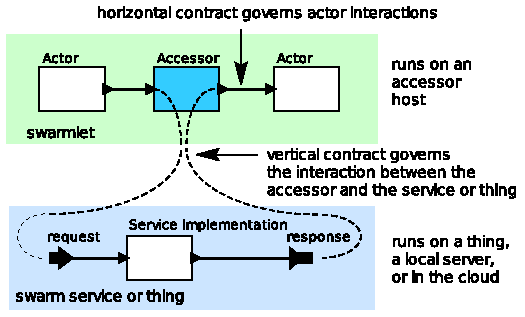
\includegraphics[height=0.4\textheight]{figures/accessors.pdf}
      \caption{Accessor in a network of actors.}
    \end{subfigure}
    \hfill
    \begin{subfigure}{0.49\textwidth}
      \centering
      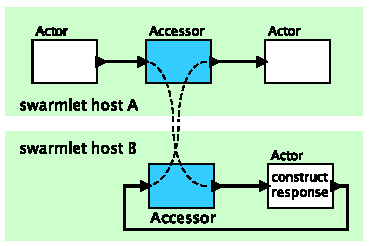
\includegraphics[height=0.4\textheight]{figures/accessors2.pdf}
      \caption{Instantiate accessors on another host.}
    \end{subfigure}
  \end{figure}

  \pause
  Look forward to Marten's dissertation talk :)
\end{frame}

\begin{frame}[standout]
  \begin{columns}
    \column{0.5\textwidth}
    \centering
    1N73LL1G3NC3 \\
    15 7H3 \\
    4B1L17Y \\
    70 4D4P7 70 \\
    CH4NG3
    \pause
    \column{0.5\textwidth}
    \begin{figure}
      \centering
      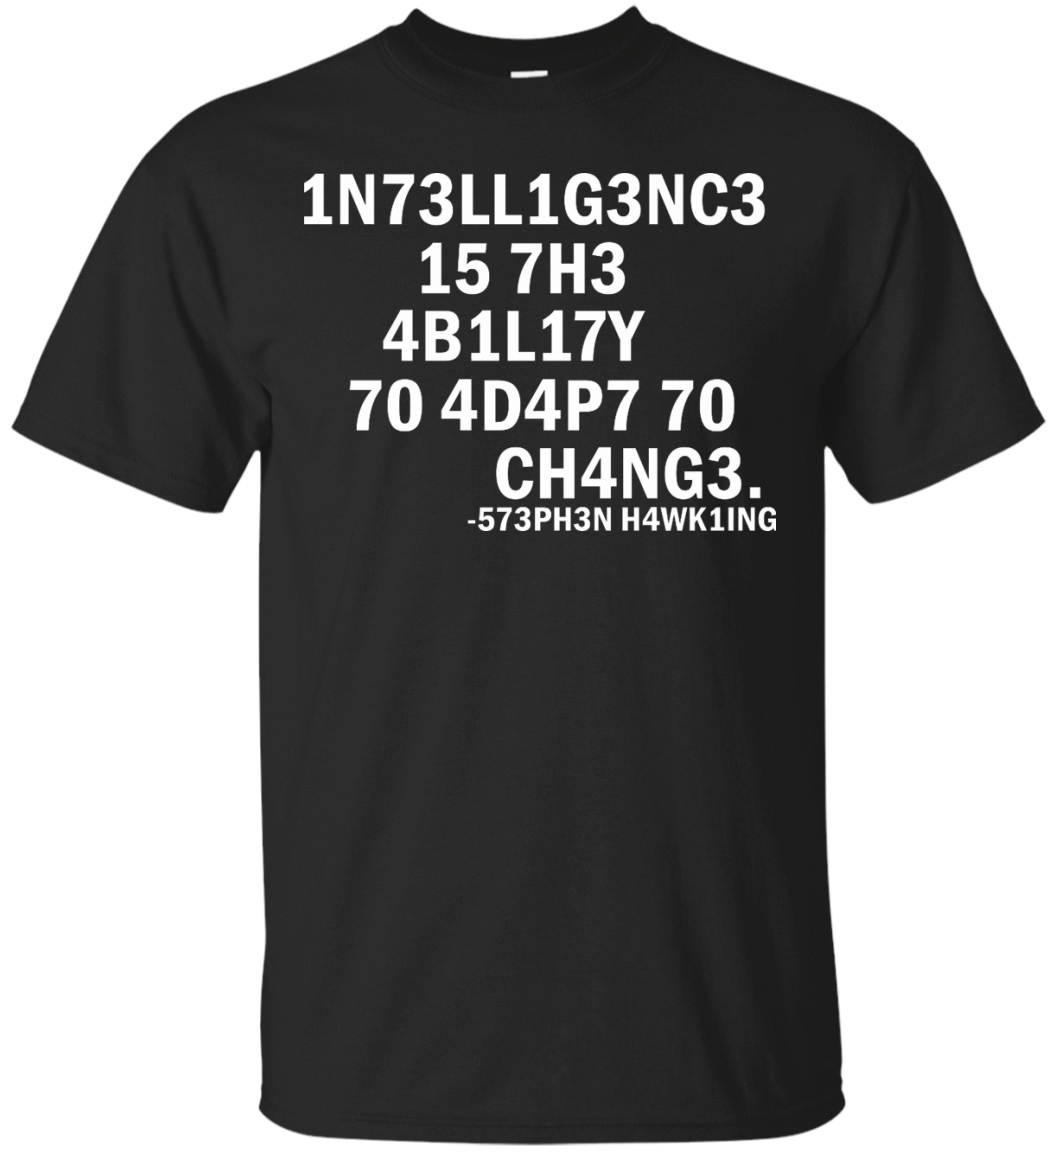
\includegraphics[height=\textwidth]{figures/shirt.png}
      \caption{\color{white} Image Source: \href{https://www.0stees.com/products/intelligence-is-the-ability-to-adapt-to-change-shirt-hoodie-tank?variant=40350207242}{0stees.com}}
    \end{figure}
  \end{columns}
\end{frame}

%%% Local Variables:
%%% mode: latex
%%% TeX-master: "../talk"
%%% TeX-engine: xetex
%%% End:
